\documentclass[12pt]{article}
\usepackage[utf8]{inputenc}
\usepackage[auth-lg]{authblk}
\usepackage[margin=1.0in]{geometry}
\usepackage[]{graphicx}
\usepackage[]{ctable}
\usepackage[]{natbib}
\usepackage[]{array}
\usepackage[]{bm}
\usepackage[]{float}
\newcolumntype{P}[1]{>{\centering\arraybackslash}p{#1}}

\title{Benchmarking Current RNA Folding Software and Improvements to the Current Regime}

\begin{document}
\author{Jianglin Liu}
\author{Bingxi Li}
\author{Gregory Rehm}
\affil{\normalsize{University of California, Davis}
\{\texttt{jiliu, bxli, grehm\}@ucdavis.edu}}
\maketitle

\begin{abstract}
Finding the secondary structure of RNA is important for understanding how RNA
will interact in a cell. Frequently computational algorithms are used to determine
structure due to difficulties extracting good \textit{in vivo} data of RNA
structures. Many of the algorithms for RNA folding are computationally complex.
In this paper we establish benchmarks for two commonly used RNA folding packages,
mfold, and RNAfold Vienna, and compare them to an improved Four-Russians folding
algorithm. We show \textit{RNAfold Vienna} is superior to mfold when evaluating RNA
strands of 900 nucleobases and less but \textit{mfold} is superior to RNAfold Vienna for
evaluating circular RNA of 1000 nucleobases. We also show that these software
packages would benefit greatly from using new improved RNA folding algorithms especially for strands
of RNA greater than 1000 nucleobases. These results will help software maintainers to understand
the benefit of updating their algorithms. The results will also help guide users
when choosing RNA folding software when looking for the most computationally optimal package.
\end{abstract}
\section{Introduction}
\par RNA is an essential macromolecule used in protein formation and performs
other essential functions within the body\cite{turner}. RNA does not stay in
single stranded form and instead folds on itself to create the lowest energy
conformation possible to ensure thermodynamic stability\cite{herschlag}. When
folding, RNA forms a 2D secondary structure\cite{mccaskill} with A matching to U
and G to C (figure 1).  Using this data we can find a 3D tertiary structure\cite{mccaskill}.
\begin{figure}[ht!]
  \centering
  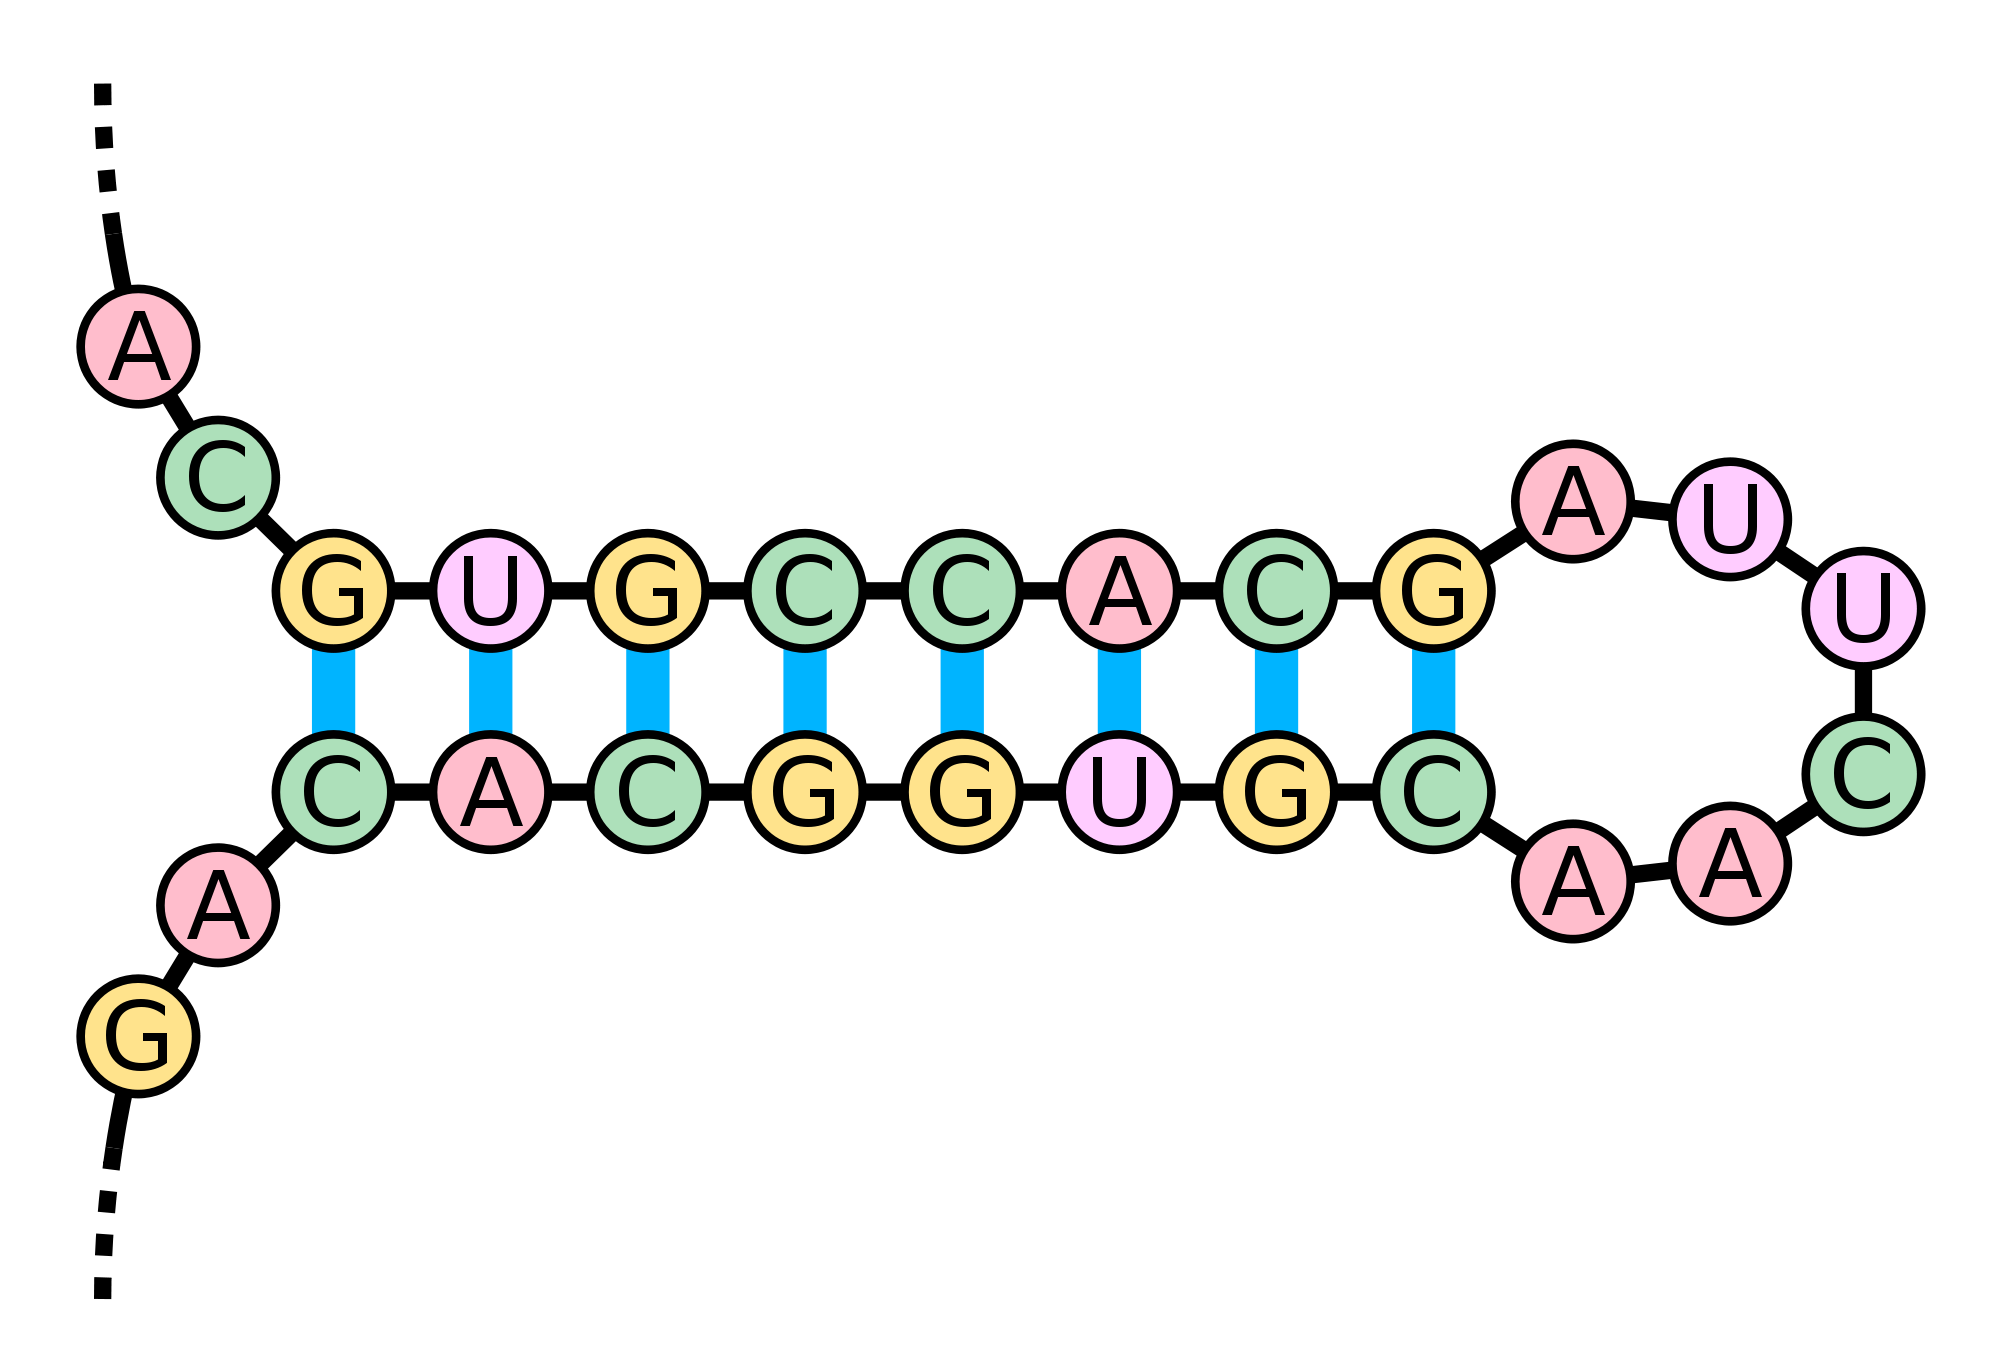
\includegraphics[keepaspectratio, scale=0.12]{fold-example.png}
  \caption{Example of an RNA molecule folding}
  \label{fig:RNA Folding}
\end{figure}
\par Our paper focuses on benchmarking 2D secondary structure prediction software
based off the Nussinov dynamic programming algorithm\cite{nussinov} for RNA folding.
This algorithm is $O(n^3)$ time complexity. There have been multiple attempts to
parallelize the Nussinov algorithm\cite{rizk, other-gpu} which have resulted in
large speed increases, however, CPU intensive algorithms only slightly lowered
the bound up until 2010\cite{minor-nussinov-improvement, chan}. In 2010 the
Nussinov bound that was significantly improved by the Frid-Gusfield Four Russians
method which established you could perform the DP method in $O(\frac{n^3}{log(n)})$
time\cite{gusfield}. Later a parallel method of the Four Russians algorithm
presented proof that you can lower this bound to $O(\frac{n^2}{log(n)})$ inside
an NVIDIA CUDA environment\cite{balaji}.
\par There are two major RNA folding software packages, mfold\cite{zuker1989,zuker1981},
and the Vienna RNA Package\cite{vienna}. These both utilize the Nussimov method
to return results of the RNA secondary structure by finding the lowest possible
thermodynamic conformations of the RNA\cite{zuker1981,vienna}. In order to tell
which was faster we performed application level benchmarks\cite{eulogy} to see
which of these two applications could more quickly fold RNA of
the circular and linear variety. The way mfold is written allows linear RNA to
be treated as exceptional variants of circular ones\cite{circular}. RNAfold
Vienna was initially optimized to only handle linear RNA\cite{circular} but
later improvements enabled it to speed the folding of circular ones\cite{circular}.
As a result we wished to determine what kind of speed difference still exists
between mfold and Vienna when performing analysis on circular RNA. To see how
these folding applications could benefit from replacing their use of the Nussinov
method with newer ones we then performed micro-benchmarks\cite{sysperformance} of the Nussinov,
the serial Frid-Gusfield method, and the parallel Four Russians method.

\par Our main finding when performing application benchmarks on mfold and
Vienna was that Vienna is significantly faster than mfold for linear and cicular
RNA strands of 900 nucleobases. For micro-benchmarks we found that the Frid Gusfield method
returned results much faster than the Nussinov method especially for larger strands of RNA. However
the parallel Four Russians CUDA algorithm returned results significantly quicker than the other serial
methods. The results of the micro-benchmarks show that both mfold and RNAfold Vienna could experience
significant speed increases if they implemented the Frid-Gusfield method. Furthermore
the authors of this paper would recommend both software packages to support GPU
hardware to achieve even greater speed gains when inside a parallel capable
environment.

\section{Methods}
\subsection{Standardizing the Testing Environment}
Benchmarking is renown as a difficult thing to perform effectively\cite{sysperformance,eulogy}.
There are many processes that can be executing on a computer at any one moment
that it is possible that a benchmark can give inaccurate information due to
conflicting processes running in the background\cite{sysperformance}. As a result
we used a machine solely dedicated for benchmarking and no other tasks. We also
standardized on the following specifications for our runs\cite{benchspecs}:
\begin{center}
    \begin{tabular}{P{5.0cm}P{3.5cm}P{3.0cm}}
        \specialrule{.1em}{.05em}{.05em}
        \textbf{Architecture} & \textbf{Operating System} & \textbf{Compiler} \\ \hline
        8 core Intel i7 CPU 4.00 GHz 16G RAM GeForce GTX 960 & Linux 4.2.5-201 Fedora 22 & GCC 5.1.1-4.fc22 \\ \hline
        " & " & gcc-gfortran 5.1.1-4.fc22\\ \hline
        " & " & NVIDIA CUDA version 5.5 \\
        \specialrule{.1em}{.05em}{.05em}
    \end{tabular}
\end{center}
We used the following applications with corresponding versions and requirements in our test runs:
\begin{center}
    \begin{tabular}{ccc}
        \specialrule{.1em}{.05em}{.05em}
        \textbf{Application} & \textbf{Version} & \textbf{Requirements} \\ \hline
        mfold & 3.6 & GCC, Fortran \\ \hline
        RNAfold Vienna  & 2.1.9 & GCC \\ \hline
        Frid-Gusfield Four Russians & N/A & GCC \\ \hline
        Parallel Four Russians & N/A & GCC, NVIDIA CUDA \\
        \specialrule{.1em}{.05em}{.05em}
    \end{tabular}
\end{center}
\par Our testing architecture was laid out where we would SSH into the benchmarking
machine and then execute tests. Test results would then be reported back to the
user's central machine where they could be stored in a database for later analysis
(figure 2). Our testing required no internet connectivity besides the ssh access
required to initiate our testing so all calculations were performed locally. Also
there were no IO operations except for post processing of mfold and Vienna results.
\begin{figure}[ht!]
  \centering
  \includegraphics[keepaspectratio, scale=0.7]{benchmarking-architecture.png}
  \caption{Test Architecture}
  \label{fig:Testing Arch}
\end{figure}

\subsection{Data Inputs}
\par For input data we give inputs of RNA as strings in a file. An example of this
would be the 10 character RNA string AUGCCAUGGA. This same RNA sequence can be
treated as circular by providing parameters to the mfold and RNAfold Vienna
programs that tell it the RNA is circular\cite{mfold-manual, vienna-manual}.
\subsection{Application Benchmarks}
\par The first type of benchmark we perform is the application level benchmark.
An application benchmark is designed to measure the performance of an entire
application and the resources it consumes on an individual machine\cite{jain}.
In our case we wish to evaluate the amount of time that mfold and RNAfold Vienna
take to return RNA secondary structures given different length RNA strands varying
on linear and circular variety. Since a single run of an application may vary in
time even for identical inputs. Because of this we evaluate each input of RNA 30
times and report the mean $\mu$, standard deviation, $\sigma^2$, of the runs
corresponding to each sequence length.

\subsection{Micro-benchmarks}
\par The most basic type of benchmark to perform is the micro-benchmark. The
micro-benchmark is a single piece of code executed many times in serial so that
we can get a profile of its run characteristics\cite{eulogy,sysperformance}.
Once these characteristics are observed we can then make inferences about its
performance and ways that it can be improved.
\par Micro-benchmarks have the downside
of losing generality of performance across the entire application\cite{eulogy, sysperformance}.
A good example of this is if an IO heavy function made many consecutive calls to
the \textit{read} function on the OS while the rest of the application made no
calls to \textit{read} whatsoever. If we tried to generalize this one function to
the rest of the application we would misguidedly attempt to optimize disk IO
across our entire system.
\par We avoid this trap in our paper by benchmarking only parts of the code that
execute the Nussinov algorithm in mfold and the Vienna package. We then report
these results back to our test results database for later analysis. After this we
compare these results to runs of the serial Frid-Gusfield algorithm and parallel
Frid-Gusfield algorithm.

\subsection{Frid-Gusfield Four-Russians Algorithm}
\par The Four-Russians Algorithm \cite{gusfield} is an algorithm to improve the
above-mentioned Nussinov $O(n^3)$ Algorithm by Four-Russian method. The Frid and Gusfield
is an $O(\frac{n^3}{\log n})$ algorithm. The Four Russian algorithm achieves this
speed up by understanding that we can make certain optimizations to the matrix of
matching base pairs required by the Nussinov algorithm. Particularly, the values
along a column from bottom to top and along a row from left to right are monotonically
non-decreasing. Consecutive cells differ at most by 1\cite{gusfield}. As a result we can
perform pre-processing of specific operations that the Nussinov algorithm must compute manually.

\subsection{CUDA Parallel Implementation for F-G Method}
\par Compute Unified Device Architecture (CUDA) is a parallel computing platform created by NVIDIA. By using CUDA API, Venkatachalam presented an $O(\frac{n^2}{logn})$ algorithm for RNA folding is presented \cite{balaji}. The CUDA implementation parallelizes the two-vector method so that achieve an enhancement of another factor of $O(n)$.

\section{Results}

\subsection{Application Benchmarks}
\par In this part, we performed the benchmark for two packages using the Dynamic Programing (DP) paradigm with
both linear and circular RNA. We report the number of RNA bases or \textbf{size}, the number of times the folding
program was run with our specific input or \textbf{N runs}, the mean timing of the runs as \boldsymbol{$\mu$}, and the standard deviation of the
runs denoted as \boldsymbol{$\sigma^2$}. For the benchmarking of both linear and circular types of RNA, we select the RNA of the size,
ranging from 200 nucleobases to 1000 nucleobases. The time to fold these structures are compared in the following Table 1.
\begin{table}[h!]
    \begin{tabular}{ |p{1.5cm}||p{1.05cm}|p{1.05cm}|p{1.05cm}|p{1.05cm}|p{1.05cm}|p{1.05cm}|p{1.05cm}| p{1.05cm} | p{1.05cm} |}
    \hline
    \multicolumn{10}{|c|}{Timing of \textit{m-fold} package for linear RNA (sec.)} \\
    \hline
    size& 200& 300& 400& 500& 600& 700 & 800 & 900 & 1000\\
    \hline
    N runs& 30 & 30& 30 & 30& 30& 30& 30& 30& 30\\
    \hline
    $\mu$& 2.523 & 6.635 & 6.313 & 8.336 & 10.492 & 9.384 & 12.212 & 14.319 & 14.402\\
    $\sigma^2$ &0.343 & 0.251 & 0.180 & 0.547 & 0.144 & 0.094 & 0.176 & 0.118 & 0.211 \\
    \hline
    \end{tabular}

    \begin{tabular}{ |p{1.5cm}||p{1.05cm}|p{1.05cm}|p{1.05cm}|p{1.05cm}|p{1.05cm}|p{1.05cm}|p{1.05cm}| p{1.05cm} | p{1.05cm} |}
    \hline
    \multicolumn{10}{|c|}{Timing of $Vienna$ for linear RNA (sec.)} \\
    \hline
    size& 200& 300& 400& 500& 600& 700 & 800 & 900 & 1000\\
    \hline
    N runs& 30 & 30& 30 & 30& 30& 30& 30& 30& 30\\
    \hline
    $\mu$& 0.029 & 0.072 & 0.112 & 0.163 & 0.508 & 0.491 & 1.934 & 11.723 & 8.296\\
    $\sigma^2$ &0.006 & 0.001 & 0.001 & 0.001 & 0.002 & 0.002 & 0.006 & 0.336 & 0.011 \\
    \hline
    \end{tabular}
\caption{The time taken by two packages to predict secondary structures of linear RNA of different length.}
\end{table}

\begin{figure}[H]
    \centering
    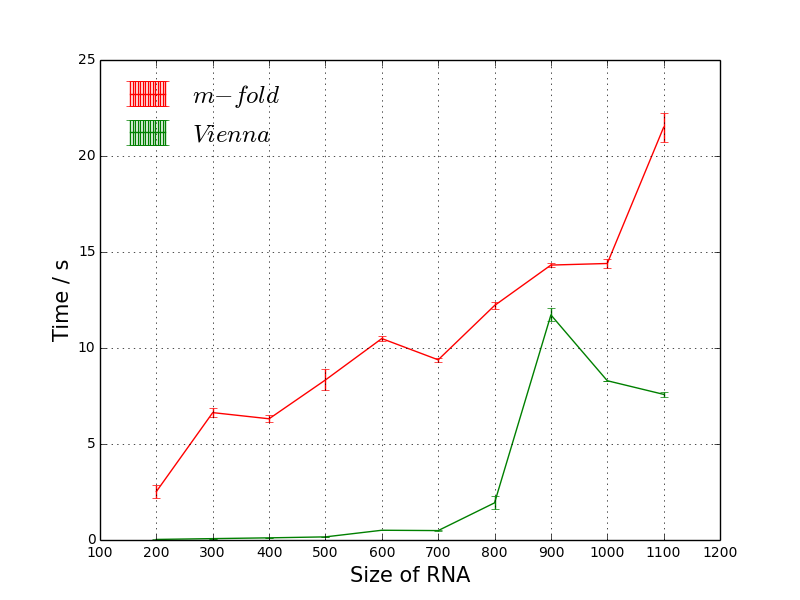
\includegraphics[width=0.75\textwidth]{l-m-v.png}
    \caption{Benchmark of \textit{Vienna} and \textit{m-fold} packages with linear RNA of different sizes.}
    \label{fig:linear}
\end{figure}

We can see from Figure \ref{fig:linear}. that \textit{m-fold} takes the most time to complete. However as mentioned before, Vienna
is optimized to handle linear RNA so these results are not necessarily surprising.
We benchmark circular RNA. The execution time to determine their secondary structures are listed in the following Table 2.

\begin{table}[H]
\begin{center}
    \begin{tabular}{ |p{1.5cm}||p{1.05cm}|p{1.05cm}|p{1.05cm}|p{1.05cm}|p{1.05cm}|p{1.05cm}|p{1.05cm}| p{1.05cm} | p{1.05cm} |}
    \hline
    \multicolumn{10}{|c|}{Timing of \textit{m-fold} package for circular RNA (sec.)} \\
    \hline
    Size& 200& 300& 400& 500& 600& 700 & 800 & 900 & 1000\\
    \hline
    N runs& 30 & 30& 30 & 30& 30& 30& 30& 30& 30\\
    \hline
    average& 2.409 & 6.633 & 6.269 & 8.889 & 11.274 & 9.074 & 11.358 & 14.678 &16.712\\
    std ($\sigma^2$) & 0.060 & 0.354 & 0.362 & 0.159 & 0.1176 & 0.161 & 0.364 & 0.1999 & 0.285 \\
    \hline
    \end{tabular}
    \begin{tabular}{ |p{1.5cm}||p{1.05cm}|p{1.05cm}|p{1.05cm}|p{1.05cm}|p{1.05cm}|p{1.05cm}|p{1.05cm}| p{1.05cm} | p{1.05cm} |}
    \hline
    \multicolumn{10}{|c|}{Timing of \textit{Vienna} for circular RNA (sec.)} \\
    \hline
    Size& 200& 300& 400& 500& 600& 700 & 800 & 900 & 1000\\
    \hline
    N runs& 30 & 30& 30 & 30& 30& 30& 30& 30& 30\\
    \hline
    average& 0.027 & 0.084 & 0.129 & 0.153 & 0.664 & 0.351 & 1.943 & 7.915 & 50.15\\
    std ($\sigma^2$) & 0.002 & 0.001 & 0.001 & 0.002 & 0.002 & 0.002 & 0.006 & 0.036 & 0.126 \\
    \hline
    \end{tabular}
\caption{The time taken by two packages to predict secondary structures of circular RNA of different length.}
\end{center}
\end{table}
\begin{figure}[H]
    \centering
    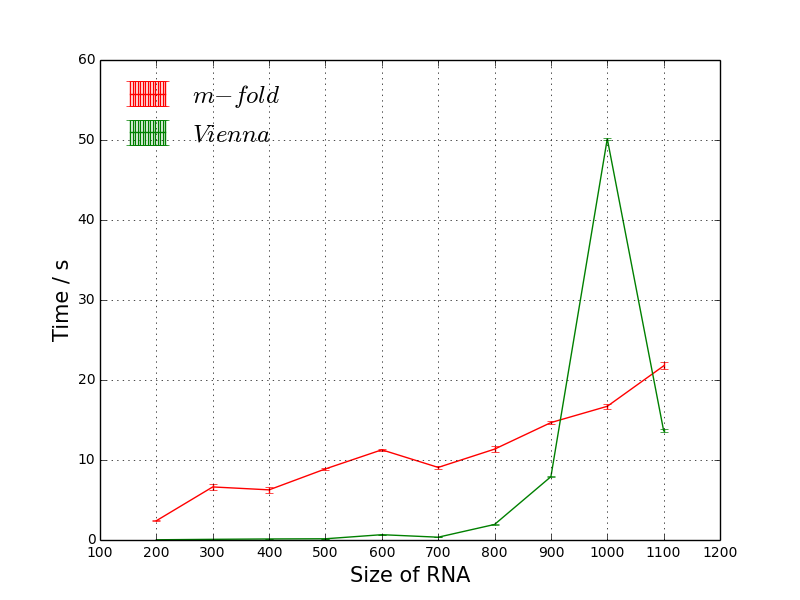
\includegraphics[width=0.75\textwidth]{c-m-v.png}
    \caption{Benchmark of \textit{Vienna} and \textit{m-fold} with circular RNA of different sizes.}
    \label{fig:circular}
\end{figure}
As we can see from Figure \ref{fig:circular} Vienna initially outperforms \textit{m-fold} but as RNA size hits 1000 bases the time to
complete the folding increases dramatically. So it appears the optimizations made to Vienna by Hofacker and
Stadler\cite{circular} break down around 1000 nucleobases.

\subsection{Micro-benchmarks}
The timing for Nussinov, Frid-Gusfield (FG), and CUDA Four-Russian algorithms are listed below with different sizes of RNA sequences 500 to 6000. The data is presented in Table ~\ref{table:timingAlgorithm}.\\
\begin{table}[H]
\begin{center}
    \begin{tabular}{ |p{1.5cm}||p{1.2cm}|p{1.3cm}|p{1.3cm}|p{1.4cm}|p{1.4cm}|p{1.4cm}|p{1.6cm}|}
     \hline
     \multicolumn{8}{|c|}{Timing of Algorithms for RNA Folding (sec.)} \\
     \hline
     size& 500& 1000& 2000& 3000& 4000& 5000& 6000\\
     \hline
     Nussinov& 0.2790& 2.0751& 16.7033& 57.8146& 145.2998& 301.4874& 519.6531\\
     F-G& 0.0903& 0.6092& 5.5868& 19.6117& 49.3309& 95.6461& 162.9072\\
     CUDA& 0.0088& 0.1988& 0.4690& 1.1943& 2.5817& 4.8506& 8.2735\\
     \hline
    \end{tabular}
\end{center}
\caption{The time take by \textit{Nussinov}, \textit{F-G} and \textit{CUDA} to construct the secondary structures of RNA of different size.}
\label{table:timingAlgorithm}
\end{table}
\par By plotting Figure \ref{fig:timingAlgorithm}, we observe the \textit{F-G} method has a vast advantage
over \textit{Nussinov} when the size of RNA sequence is larger than 3000, and the \textit{CUDA} method
becomes much more useful around this point as well.
\begin{figure}[H]
  \centering
  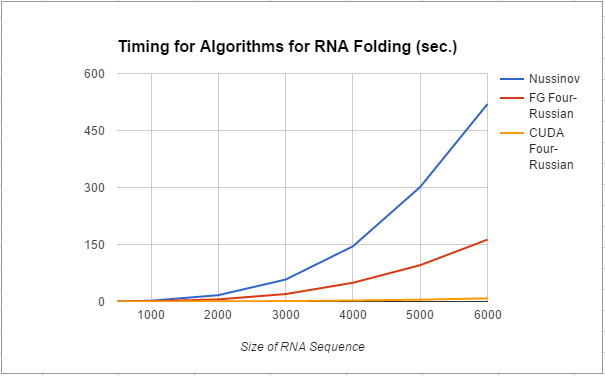
\includegraphics[keepaspectratio, scale=.6]{algorithmGraph.png}
  \caption{Timing of Algorithms for RNA Folding (sec.)}
  \label{fig:timingAlgorithm}
\end{figure}

\section{Conclusion and Discussion}
\par In this paper, we performed application benchmarks for \textit{m-fold} and \textit{RNAfold Vienna} and
micro-benchmarks for the Nussinov, Frid-Gusfield, and parallel Four Russians algorithms. For the
application benchmark, \textit{RNAfold Vienna} and \textit{m-fold} have been applied to predict
the secondary structure of both linear and circular RNA. In both linear and circular cases, the
\textit{Vienna} package is clearly optimal for chains of RNA smaller than 900 bases.  While
\textit{m-fold} is time optimal in the prediction of circular RNA structures of 1000 nucleobases and likely
for circular RNA strands of greater than 1000 nucleobases, although more testing is necessary to establish this conclusively.

\par When we come to the micro-benchmarks, we found that the \textit{Nussinov} DP method becomes
appreciably slower, particularly to the human user, in the cases that the number of nucleotides in the RNA sequence is
greater than 1000. This is intrinsically caused by the fact the algorithm is of $O(log(n^3))$ time complexity.
Furthermore, while the \textit{Frid-Gusfield} method \cite{gusfield} has enhanced the performance by a factor of $log(n)$,
in cases where RNA strands are greater than 2000 nucleobases speed is still not satisfactory. With the introduction
of \textit{CUDA} using the two-vector method invented by Venkatachalam\cite{balaji}, we achieve a much closer
to linearly increasing time complexity for different sizes of RNA sequences. Thus when dealing with super long RNA
sequences of greater than 2000 nucleobases investing in the use of parallel algorithms and CUDA becomes much
more cost effective especially if we consider that we would be waiting 519 seconds just to run an RNA sequence
through the Nussinov method.

\par For future work we wish to benchmark \textit{RNAfold Vienna} and \textit{mfold} for RNA sequences
greater than 1000 nucleobases. We have some evidence now that \textit{m-fold} is superior to Vienna when
predicting secondary structures of RNA greater than 1000 nucleobases however we do not know if this will
continue to hold. Furthermore we'd also like to know with better exactitude the length of nucleobases at which
the performance between the two applications differs. Another excellent experiement would be to understand which
types of RNA sequences do the respective applications deal with more effectively. For our experiment we only
used a single RNA sequence for each length but future experiments can involve multiple random RNA sequences
of the same length. This way we can obtain a more interesting standard deviation of timing compared to what
we have found in this paper. We can apply the same methodology to our micro-benchmarks as well. Although results may not vary as significantly because the thermodynamic rules that \textit{Vienna} and \textit{m-fold}
employ are not present.

\par We believe that future work on integrating the Frid-Gusfield and parallel CUDA methods into \textit{m-fold} and \textit{Vienna} will be very important. RNA packages like \textit{RNAfold Vienna} and \textit{m-fold} must also
take into account complex thermodynamic rules in order to find both optimal and suboptimal RNA structures. These
caluculations all use the Nussinov method and as a result slow execution time down even more in an
application setting. As a result implementation of an improved folding algorithm like Frid-Gusfield
or the parallel Four Russians introduced by Venkatachalam is imperative especially as we discover more,
and longer chains of RNA that are biologically significant.

\section{Author Contributions}
Bingxi Li contributed to running RNAfold Vienna and providing benchmarking results. Jianglin Liu ran the
micro-benchmark algorithms and provided results. Gregory Rehm ran the mfold application benchmarks,
performed background research on both RNA folding software and benchmarking, and provided the run methodology
for our experiments.
\begin{thebibliography}{56}
\bibitem{gusfield}
Frid Y, Gusfield D.
\textit{A simple, practical and complete O($n^3$)-time
algorithm for RNA folding using the Four-Russians Speedup}.
Algorithms Mol Biol 2010, 5:13

\bibitem{balaji}
Venkatachalam B, Gusfield D.
\textit{Faster algorithms for RNA-folding using the Four-Russians method}.
Algorithms for Molecular Biology20149:5.

\bibitem{nussinov}
Nussinov R, Jacobson A.
\textit{Fast algorithm for predicting the secondary structure of
single-stranded RNA}.
Proc. Nati. Acad. Sci. USA Vol. 77, No. 11, pp. 6309-6313, November 1980.

\bibitem{turner}
Mathews D, Turner D.
\textit{Prediction of RNA secondary structure by free energy
minimization}.
Current Opinion in Structural Biology 2006, 16:270–278.

\bibitem{mccaskill}
McCaskill J.S.
\textit{The Equilibrium Partition Function and Base Pair
Binding Probabilities for RNA Secondary Structure.}
Biopolymers, Vol. 29,1105-1119 (1990)

\bibitem{herschlag}
Herschlag D.
\textit{RNA Chaperones and the RNA Folding Problem}.
Vol. 270, No. 36, Issue of September 8, pp. 20871–20874, 1995

\bibitem{vienna}
Hofacker I. L, Fontana W, Stadler P. F, Bonhoeffer L. S, Tacker M, Schuster P.
\textit{Fast Folding and Comparison of RNA Secondary Structures}.
Monatshefte ftir Chemie 125, 167-188 (1994)

\bibitem{zuker1989}
Zuker M.
\textit{Computer Prediction of RNA Structure}.
Methods in Enzymology, vol. 180.

\bibitem{zuker1981}
Zuker M, Steigler P.
\textit{Optimal computer folding of large RNA sequences using thermodynamics and auxiliary information}.
Nucleic Acids Research vol. 9 Number 11981.

\bibitem{sysperformance}
Gregg B.
\textit{Systems Performance; Enterprise and the Cloud}.
Pearson Education 2014 Upper Saddle River, NJ

\bibitem{benchspecs}
Altun, O.
\textit{Clustering Application Benchmark}.
IISWC.2006.302742

\bibitem{minor-nussinov-improvement}
Akutsu, T.
\textit{Approximation and Exact Algorithms for RNA
Secondary Structure Prediction and Recognition
of Stochastic Context-free Languages}
Journal of Combinatorial Optimization 3, 321–336 (1999)

\bibitem{chan}
Chan TM.
\textit{More Algorithms for All-Pairs Shortest Paths in Weighted
Graphs}.
SIAM J Comput 2010, 39(5):2075-2089

\bibitem{eulogy}
Cantrill B.
\textit{Eulogy for a benchmark}.
The Observation Deck Web. http://dtrace.org/blogs/bmc/2009/02/02/eulogy-for-a-benchmark/.
2009.

\bibitem{rizk}
Rizk G, Lavenier D.
\textit{GPU accelerated Rna folding algorithm}.
Allen, G.; Nabrzyski, J.; Seidel, E.; Albada, G.D. van; Dongarra, J.; Sloot, P.M.A. 9th International Conference on Computational Science, May 2009, Baton Rouge, United States. Springer., 5544, pp.1031, 2009, LNCS. <10.1000.ISBN: 978-3-642-01969-2>. <hal-00425543>

\bibitem{other-gpu}
Chang D, Kimmer C, Ming O.
\textit{Accelerating the Nussinov RNA Folding Algorithm with CUDA/GPU}
Signal Processing and Information Technology (ISSPIT), 2010 IEEE International Symposium on, 15-18 Dec. 2010, pp. 120-125

\bibitem{circular}
Hofacker I, Stadler P.
\textit{Memory efficient folding algorithms for circular RNA secondary structures}.
Bioinformatics (2006) 22 (10): 1172-1176.

\bibitem{mfold-manual}
Zuker M, Matthews D.H, Turner D.H.
\textit{Algorithms and Thermodynamics for RNA
Secondary Structure Prediction:
a Practical Guide}.
The mfold Web Server Web. http://unafold.rna.albany.edu/doc/mfold-manual/mfold-3.0-manual.pdf.gz.

\bibitem{vienna-manual}
Hofacker I, Fontana W, Bonhoeffer S, Stadler P.F, Lorenz R.
\textit{RNAFOLD}.
Theoretical Biochemistry Group Institute for Theoretical Chemistry Web. https://www.tbi.univie.ac.at/RNA/RNAfold.1.html\#heading5

\bibitem{jain}
Jain, R.
\textit{Art of Computer Systems Performance Analysis Techniques For Experimental Design Measurements Simulation And Modeling}.
Wiley Computer Publishing, John Wiley \& Sons, Inc.
ISBN: 0471503363 Pub Date: 05/01/91.

\end{thebibliography}

\end{document}
